\documentclass[11pt,a4paper]{article}
\usepackage[margin=2.6cm]{geometry}
\usepackage{amsmath,amssymb,amsthm}
\usepackage{tikz}
\usepackage{booktabs}
\usepackage[hidelinks]{hyperref}
\usepackage{xcolor}

\newtheorem*{paperthm}{\paperthmname}
\newcommand{\paperthmname}{}
\newtheorem{lemma}{Lemma}
\theoremstyle{remark}
\newtheorem*{example}{Worked example}
\newtheorem*{checkit}{Check it yourself}
\newcommand{\avg}[1]{\left\langle #1 \right\rangle}
\newcommand{\dd}{\mathrm{d}}
\newcommand{\nb}[1]{\texttt{validation/#1}}

\title{The pizzetti proofs, explained\\[4pt]\large Part 1: The interior series and its error bound}
\author{Companion to the pizzetti paper (Sections 2--4 and Appendix A)}
\date{}

\begin{document}
\maketitle

\begin{abstract}
\noindent This is a slow, step-by-step version of the proof that the pizzetti interior series
has a guaranteed error bound (Theorem~2 of the paper). It assumes only first-year calculus:
the binomial series, geometric series, and averaging a function over a disk. Every step comes
with a small numerical example, and every formula is checked independently in the validation
notebooks of the repository (\nb{02\_series\_theorem2.ipynb}). The paper itself is the
authoritative, terse version; nothing here goes beyond it.
\end{abstract}

\paragraph{Where is what.} The three parts of this companion follow the paper:
\begin{center}
\begin{tabular}{lll}
\toprule
Paper & Content & Here\\
\midrule
Sections 2--3, 4.1, Appendix A & interior series, Theorem 2, the cut & Part 1\\
Section 4.2, Appendix B (incl.\ B.1) & mean-value expansion, Propositions 1--2 & Part 2\\
Sections 5.1, 5.3, Appendix C & contact expansions, Theorem 3 & Part 3\\
\bottomrule
\end{tabular}
\end{center}

\tableofcontents

%% ===================================================================
\section{The question}

A star is a disk of radius 1. Its brightness drops towards the edge: at distance $r$ from the
centre the surface brightness is a sum of powers of
\[
  \mu=\sqrt{1-r^2},
\]
for example $I=1-u_1(1-\mu)-u_2(1-\mu)^2$ for the quadratic law. A planet is a dark disk of
radius $p$ (in units of the stellar radius) whose centre lies at distance $z$ from the stellar
centre (Figure~\ref{fig:geom}). While the planet lies \emph{entirely inside} the star, that is
$z+p<1$, the light it blocks is the brightness averaged over the planet's disk, times its area.
Every power $\mu^{\alpha}$ is $(1-r^2)^\gamma$ with $\gamma=\alpha/2$, so everything reduces to
one quantity, the \emph{disk average}
\begin{equation}
  D_\gamma(z,p)=\avg{(1-r^2)^\gamma}
  =\frac{1}{\pi p^2}\int_{\text{planet disk}}(1-r^2)^\gamma\,\dd A .
  \label{eq:D}
\end{equation}
For whole numbers $\gamma$ this is a polynomial and easy. For $\gamma=\tfrac12$ (the $\mu$ term
of the quadratic law) it needs elliptic integrals, and for other values such as $\gamma=0.3$ there
is no closed formula at all. The paper replaces $D_\gamma$ by a short polynomial and proves how
large the error can be. This part explains that proof.

\begin{figure}[h]
\centering
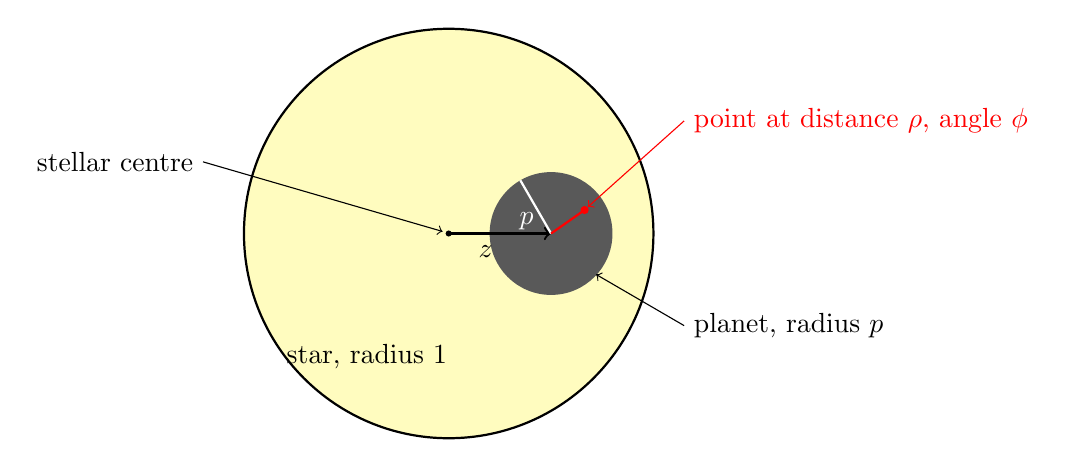
\begin{tikzpicture}[scale=2.6]
  \fill[yellow!25] (0,0) circle (1);
  \draw[thick] (0,0) circle (1);
  \fill[black!65] (0.5,0) circle (0.3);
  \draw[->,thick] (0,0) -- (0.5,0);
  \node[below] at (0.18,-0.01) {$z$};
  \draw[white,thick] (0.5,0) -- ++(120:0.3);
  \node[white] at (0.38,0.06) {$p$};
  \fill (0,0) circle (0.015);
  \draw[red,thick] (0.5,0) -- ++(35:0.2);
  \fill[red] (0.5,0) ++(35:0.2) circle (0.02);
  \draw[red,->] (1.15,0.55) node[right] {point at distance $\rho$, angle $\phi$} -- (0.68,0.13);
  \draw[->] (-1.2,0.35) node[left] {stellar centre} -- (-0.03,0.01);
  \draw[->] (1.15,-0.45) node[right] {planet, radius $p$} -- (0.72,-0.2);
  \node at (-0.4,-0.6) {star, radius 1};
\end{tikzpicture}
\caption{A planet of radius $p$ at distance $z$ from the stellar centre. A point of the planet's
disk is described by its distance $\rho\le p$ from the planet's centre and an angle $\phi$.}
\label{fig:geom}
\end{figure}

%% ===================================================================
\section{Step 1: Pull out the value at the planet's centre}

A point of the planet's disk at distance $\rho$ from the planet's centre, at angle $\phi$, has
squared distance from the stellar centre
\[
  r^2=z^2+2z\rho\cos\phi+\rho^2
\]
(the law of cosines). Write $w=1-z^2$: this is $1-r^2$ at the planet's centre. Then
\begin{equation}
  1-r^2=w-(2z\rho\cos\phi+\rho^2)=w\,(1-\varepsilon),\qquad
  \varepsilon=\frac{2z\rho\cos\phi+\rho^2}{w}.
  \label{eq:eps}
\end{equation}
So $(1-r^2)^\gamma=w^\gamma(1-\varepsilon)^\gamma$. The factor $w^\gamma$ is the brightness at the
planet's centre; $\varepsilon$ measures how much the brightness at the point differs from it.

\paragraph{How large can $\varepsilon$ be?} Since $|\cos\phi|\le1$ and $\rho\le p$,
\begin{equation}
  |\varepsilon|\le\varepsilon_{\max}=\frac{2zp+p^2}{1-z^2}.
  \label{eq:emax}
\end{equation}
And $\varepsilon_{\max}<1$ exactly when $2zp+p^2<1-z^2$, i.e.\ $(z+p)^2<1$, i.e.\ when the planet
lies inside the star. That is the condition we need below.

\begin{example}
Throughout this part we use $\gamma=\tfrac12$, $p=0.1$, $z=0.5$. Then $w=0.75$ and
$\varepsilon_{\max}=(0.1+0.01)/0.75=0.14\overline{6}$.
\end{example}

%% ===================================================================
\section{Step 2: Expand in powers of $\varepsilon$}

For $|\varepsilon|<1$ the binomial series gives
\begin{equation}
  (1-\varepsilon)^\gamma=\sum_{m=0}^\infty\beta_m\,\varepsilon^m,\qquad
  \beta_m=(-1)^m\binom{\gamma}{m}=\frac{(-1)^m}{m!}\,\gamma(\gamma-1)\cdots(\gamma-m+1).
  \label{eq:beta}
\end{equation}
For $\gamma=\tfrac12$ this is the familiar
$\sqrt{1-\varepsilon}=1-\tfrac12\varepsilon-\tfrac18\varepsilon^2-\tfrac1{16}\varepsilon^3-\tfrac{5}{128}\varepsilon^4-\dots$

Two facts about the coefficients carry the whole proof.

\paragraph{Fact 1 (one sign).} Going from $\beta_m$ to $\beta_{m+1}$ multiplies by
\begin{equation}
  \frac{\beta_{m+1}}{\beta_m}=-\frac{\gamma-m}{m+1}=\frac{m-\gamma}{m+1}.
  \label{eq:ratio}
\end{equation}
Once $m>\gamma$ this ratio is positive, so from there on \emph{all coefficients have the same
sign}. For $0<\gamma<1$ that happens already at $m=1$: every $\beta_m$ with $m\ge1$ is negative
(as in the $\sqrt{1-\varepsilon}$ series above). For a general non-integer $\gamma$ the common sign
is $(-1)^{\lceil\gamma\rceil}$, where $\lceil\gamma\rceil$ is $\gamma$ rounded up.

\paragraph{Fact 2 (shrinking).} For $m>\gamma$ the ratio \eqref{eq:ratio} is also less than 1,
because $m-\gamma<m+1$. So $|\beta_{m+1}|<|\beta_m|$: the coefficients shrink.

(For whole numbers $\gamma$ the factor $\gamma-m$ eventually vanishes and the series stops; that
is why integer exponents are easy.)

%% ===================================================================
\section{Step 3: Average each power over the disk}

We now average term by term over the planet's disk:
\begin{equation}
  D_\gamma=w^\gamma\sum_{m=0}^\infty\beta_m\avg{\varepsilon^m}.
  \label{eq:series}
\end{equation}

\paragraph{Why we may average term by term.} On the disk $|\varepsilon|\le\varepsilon_{\max}<1$.
Let $m_0$ be the first index above $\gamma$; from there on the coefficients shrink (Fact 2), so
every term with $m\ge m_0$ is at most $|\beta_{m_0}|\,\varepsilon_{\max}^m$ in size. The tail of the
series after $m$ terms is therefore smaller than the geometric tail
$|\beta_{m_0}|\,\varepsilon_{\max}^{m}/(1-\varepsilon_{\max})$ \emph{at every point of the disk at
once}. Averaging a sum whose tail is uniformly small is the same as
summing the averages. (In the language of analysis: the series converges uniformly, so it can be
integrated term by term.)

\paragraph{The averages $\avg{\varepsilon^m}$ are simple.} Expand
$(2z\rho\cos\phi+\rho^2)^m$ with the binomial theorem and average over the disk, where
$\dd A=\rho\,\dd\rho\,\dd\phi$. Two elementary averages are needed:
\begin{itemize}
  \item the average of $\cos^l\phi$ over a full turn is $\binom{l}{l/2}2^{-l}$ for even $l$
        (for instance $\tfrac12$ for $l=2$, $\tfrac38$ for $l=4$) and $0$ for odd $l$;
  \item the average of $\rho^n$ over the disk is $2p^n/(n+2)$.
\end{itemize}
Collecting terms gives Lemma~1 of the paper:
\begin{equation}
  \avg{\varepsilon^m}=\frac{1}{w^m}\sum_{\substack{l=0\\l\text{ even}}}^m G_{m,l}\,z^l p^{2m-l},
  \qquad G_{m,l}=\binom{m}{l}\binom{l}{l/2}\frac{2}{2m-l+2}.
  \label{eq:moments}
\end{equation}
For example
\[
  \avg{\varepsilon}=\frac{p^2/2}{w},\qquad
  \avg{\varepsilon^2}=\frac{z^2p^2+p^4/3}{w^2}.
\]
(Check the second one by hand: $\varepsilon^2w^2=4z^2\rho^2\cos^2\phi+4z\rho^3\cos\phi+\rho^4$;
the middle term averages to zero, $\avg{\rho^2}=p^2/2$, $\avg{\cos^2\phi}=\tfrac12$ and
$\avg{\rho^4}=p^4/3$.)

\paragraph{Fact 3 (never negative).} Only even powers of $\cos\phi$ survive the averaging, and
every surviving term in \eqref{eq:moments} is positive. So
\[
  \avg{\varepsilon^m}\ge0\qquad\text{for every }m.
\]
This is not obvious from the start, since $\varepsilon$ itself is negative on part of the disk
(where $\cos\phi<0$).

\begin{example}
For $\gamma=\tfrac12$, $p=0.1$, $z=0.5$ the terms $w^\gamma\beta_m\avg{\varepsilon^m}$ of
\eqref{eq:series} are
\[
\begin{array}{c|cccccc}
 m & 0 & 1 & 2 & 3 & 4 & 5\\\hline
 \text{term} & 0.866025 & -2.89\times10^{-3} & -4.88\times10^{-4} & -6.45\times10^{-6} & -1.42\times10^{-6} & -4.78\times10^{-8}
\end{array}
\]
They fall off quickly, and after the first all have the same sign (Facts 1 and 3). The exact
value, from the defining integral, is $D_{1/2}=0.86264319100026\ldots$
\end{example}

%% ===================================================================
\section{Step 4: Cut the series off and bound what is left}

Keep the terms up to $m=M$:
\[
  S_M=w^\gamma\sum_{m=0}^{M}\beta_m\avg{\varepsilon^m}.
\]
What is left over is the \emph{remainder}
\[
  D_\gamma-S_M=w^\gamma\sum_{m=M+1}^\infty\beta_m\avg{\varepsilon^m}.
\]

\renewcommand{\paperthmname}{Theorem 2 (as in the paper)}
\begin{paperthm}
Let $z+p<1$, let $\gamma>0$ not be a whole number, and let $M$ be odd with $M+1>\gamma$. Then
\begin{equation}
  |D_\gamma-S_M|\le B_M=\frac{w^\gamma\,|\beta_{M+1}|\,\avg{\varepsilon^{M+1}}}{1-\varepsilon_{\max}},
  \label{eq:bound}
\end{equation}
and the remainder $D_\gamma-S_M$ has the sign $(-1)^{\lceil\gamma\rceil}$.
\end{paperthm}

\begin{proof}[Proof, one idea at a time]
\emph{(a) All remainder terms have the same sign.} Every $m$ in the remainder satisfies
$m\ge M+1>\gamma$, so all $\beta_m$ there have the common sign $(-1)^{\lceil\gamma\rceil}$
(Fact 1), and all $\avg{\varepsilon^m}\ge0$ (Fact 3). A sum of terms of one sign has that sign,
and its size is the sum of the sizes:
\[
  |D_\gamma-S_M|=w^\gamma\sum_{m\ge M+1}|\beta_m|\,\avg{\varepsilon^m}.
\]
\emph{(b) Replace each coefficient by the first one.} The coefficients shrink (Fact 2), so
$|\beta_m|\le|\beta_{M+1}|$ for all $m\ge M+1$.

\emph{(c) Compare each average with the first one.} Here is where $M$ odd is used. Since $M+1$
is even, $\varepsilon^{M+1}=|\varepsilon|^{M+1}$. For $m\ge M+1$, at every point of the disk,
\[
  \varepsilon^m\le|\varepsilon|^m=|\varepsilon|^{M+1}\,|\varepsilon|^{m-M-1}
  \le\varepsilon^{M+1}\,\varepsilon_{\max}^{\,m-M-1},
\]
and averaging keeps the inequality:
$\avg{\varepsilon^m}\le\varepsilon_{\max}^{\,m-M-1}\avg{\varepsilon^{M+1}}$.

\emph{(d) Add up.} Putting (b) and (c) into (a),
\[
  |D_\gamma-S_M|\le w^\gamma|\beta_{M+1}|\avg{\varepsilon^{M+1}}
  \bigl(1+\varepsilon_{\max}+\varepsilon_{\max}^2+\dots\bigr)
  =\frac{w^\gamma|\beta_{M+1}|\avg{\varepsilon^{M+1}}}{1-\varepsilon_{\max}},
\]
the sum of a geometric series with ratio $\varepsilon_{\max}<1$.
\end{proof}

\paragraph{Why the bound is so close to the true error.} The bound is the first omitted term
divided by $1-\varepsilon_{\max}$. The true remainder is the first omitted term \emph{plus} smaller
terms of the same sign. When the terms fall off quickly, both are close to the first omitted term.

\begin{example}
For $\gamma=\tfrac12$, $p=0.1$, $z=0.5$:
\[
\begin{array}{c|ccc}
 M & D_{1/2}-S_M & B_M & \text{error}/\text{bound}\\\hline
 1 & -4.95\times10^{-4} & 5.71\times10^{-4} & 0.87\\
 3 & -1.47\times10^{-6} & 1.66\times10^{-6} & 0.89\\
 5 & -9.50\times10^{-9} & 1.05\times10^{-8} & 0.91
\end{array}
\]
The remainder is negative, as predicted by the sign $(-1)^{\lceil1/2\rceil}=-1$, and always below
the bound.
\end{example}

\begin{checkit}
Notebook \nb{02\_series\_theorem2.ipynb}, cell 2b, repeats this for several exponents, radius
ratios and separations against the defining integral \eqref{eq:D}, computed by brute-force
numerical integration. In the full run (2132 cases) no remainder exceeded its bound, every sign was
as predicted, and the largest ratio of error to bound was $0.99998$.
\end{checkit}

%% ===================================================================
\section{Step 5: One cut per light curve}

\paragraph{The bound grows as the planet moves outwards.} Write the bound using
\eqref{eq:moments} as
\[
  B_M=|\beta_{M+1}|\;w^{\gamma-M-1}\sum_l G_{M+1,l}\,z^lp^{2M+2-l}\;\frac{1}{1-\varepsilon_{\max}}.
\]
As $z$ increases, $w=1-z^2$ decreases, so $w^{\gamma-M-1}$ (a negative power) increases; each
$z^l$ increases; and $\varepsilon_{\max}$ increases, so $1/(1-\varepsilon_{\max})$ increases. Every
factor grows, hence so does $B_M$.

\paragraph{Consequence.} For a given planet ($p$), order $M$ and tolerance $\tau$, there is a
largest separation $z_c$ up to which the bound stays below $\tau$, and below $z_c$ it is below
$\tau$ \emph{everywhere}. One number per light curve decides where the series may be used
(Corollary~1 of the paper). For the quadratic law the flux error is the bound times a constant
factor $p^2\Omega|u_1+2u_2|$ that depends only on the limb-darkening coefficients.

\begin{example}
Quadratic law $(u_1,u_2)=(0.4,0.25)$, $M=11$, flux tolerance $10^{-9}$: for an Earth-sized planet
($p=0.0092$) the cut lies at $z_c=0.99767\,(1-p)$, for $p=0.1$ at $z_c=0.912\,(1-p)$.
Beyond $z_c$, near the stellar edge, other methods take over (Parts 2 and 3).
\end{example}

\begin{checkit}
Notebook \nb{02\_series\_theorem2.ipynb}, cell 2c, evaluates pizzetti's series on dense grids
$0\le z\le z_c$ and compares with exoplanet-core, an implementation of the exact solution of Agol,
Luger \& Foreman-Mackey (2020). The error never exceeded the tolerance.
\end{checkit}

%% ===================================================================
\section{Step 6: Why it is fast --- the polynomial form}

Each $\avg{\varepsilon^m}$ is a polynomial in $z^2$ and $p^2$ divided by $w^m$. Substituting
$z^2=1-1/v$ with $v=1/w$ turns $S_M$ into
\[
  S_M=w^\gamma\sum_{j=0}^Ma_j(p)\,v^j,
\]
a polynomial of degree $M$ in $v$ whose coefficients $a_j$ depend only on the planet size $p$
(Equations~(13)--(14) of the paper give them explicitly). For $\gamma=\tfrac12$, $M=3$:
\[
  S_3=\sqrt w\left[1-\frac{p^2}{8}(v+v^2)+\frac{p^4}{12}v^2-\frac{p^4}{8}v^3-\frac{p^6}{64}v^3\right].
\]
For a light curve the $a_j$ are computed once. Each data point then costs one subtraction for $w$,
one division for $v$, one square root (or power) for $w^\gamma$, and $M$ multiply-adds. That is
the source of the speed-up over elliptic integrals.

\begin{checkit}
Notebook \nb{02\_series\_theorem2.ipynb}, cell 2a: the polynomial form equals the partial sum to
40 digits, and the $S_3$ formula above is exact.
\end{checkit}

%% ===================================================================
\section{Summary}

The whole argument uses four elementary facts: the brightness can be written as its value at the
planet's centre times $(1-\varepsilon)^\gamma$; the binomial coefficients eventually have one sign
and shrink; the disk averages of $\varepsilon^m$ are never negative; and a geometric series sums to
$1/(1-\text{ratio})$. Together they give an error bound that is never exceeded, is close to the
true error, and grows with $z$, so a single cut per light curve guarantees the requested accuracy.

What the proof does \emph{not} cover is rounding in double-precision arithmetic, which is checked
separately (it stays below $10^{-16}$ of the stellar flux) and is negligible compared with the
tolerances used.

\medskip\noindent\textbf{Next:} Part 2 relates the series to Pizzetti's mean-value expansion and
proves two further bounds (Appendix B of the paper). Part 3 treats the phases in which the
planet crosses the stellar edge (Section 5.3 and Appendix C).

\end{document}
